% Intended LaTeX compiler: pdflatex
\documentclass[10pt,a4paper,UTF8]{article}
\usepackage{zclorg}
\usepackage{tikztheorem}
\author{张朝龙}
\date{}
\title{向死而生 --《刀锋》}
\hypersetup{
 pdfauthor={张朝龙},
 pdftitle={向死而生 --《刀锋》},
 pdfkeywords={reading},
 pdfsubject={读《刀锋有感》},
 pdfcreator={Emacs 25.0.50.1 (Org mode 9.0.6)},
 pdflang={English}}
\begin{document}

\maketitle
\tableofcontents
\titlepic{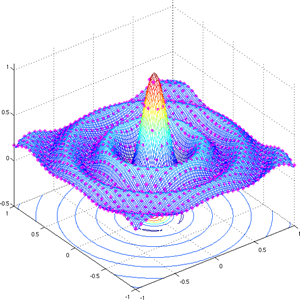
\includegraphics[scale=0.25]{../../img/sinc.PNG}}
\begin{tikzquote}


剃刀锋刃,越之维难;

智者有云,得道弥艰。
\end{tikzquote}

拉里终于找到了自己的活法:“平静节制的生活,满怀慈悲,无私忘我并禁欲克己”。如果你无法体会被问及“如何生活”,拉里说出这句活时的震撼,原谅我把拉里历经磨难的彻悟放在前面。请阅读这本小说,跟随拉里的脚步进行一段心灵的旅程。不必像拉里一样放弃所有,只需要跟随他的脚步,看着他生活,你就会慢慢有所感悟。

“我认为人类能追求的最高理性就是自我完善”,我还在自我救赎,我必须每日阅读,恰如每日进食。进食为了身体,阅读为了灵魂。我怕那天不阅读了就无法镇压内心的邪恶和贪欲,会做错事,错的自己都不知道为什么。就像望弥撒一样,阅读也是一种信仰,事关灵魂的高贵。
\end{document}
